%%%%%%%%%%%%%%%%%%%%%%%%%%%%%%%%%%%%%%%%%
% Journal Article
% LaTeX Template
% Version 1.4 (15/5/16)
%
% This template has been downloaded from:
% http://www.LaTeXTemplates.com
%
% Original author:
% Frits Wenneker (http://www.howtotex.com) with extensive modifications by
% Vel (vel@LaTeXTemplates.com)
%
% License:
% CC BY-NC-SA 3.0 (http://creativecommons.org/licenses/by-nc-sa/3.0/)
%
%%%%%%%%%%%%%%%%%%%%%%%%%%%%%%%%%%%%%%%%%

%----------------------------------------------------------------------------------------
%	PACKAGES AND OTHER DOCUMENT CONFIGURATIONS
%----------------------------------------------------------------------------------------

\documentclass[twoside]{article}

\usepackage{blindtext} % Package to generate dummy text throughout this template 

\usepackage[sc]{mathpazo} % Use the Palatino font
\usepackage[T1]{fontenc} % Use 8-bit encoding that has 256 glyphs
\linespread{1.05} % Line spacing - Palatino needs more space between lines
\usepackage{microtype} % Slightly tweak font spacing for aesthetics

\usepackage[english]{babel} % Language hyphenation and typographical rules

\usepackage[hmarginratio=1:1,top=32mm,columnsep=20pt]{geometry} % Document margins
\usepackage[hang, small,labelfont=bf,up,textfont=it,up]{caption} % Custom captions under/above floats in tables or figures
\usepackage{booktabs} % Horizontal rules in tables


\usepackage{lettrine} % The lettrine is the first enlarged letter at the beginning of the text

\usepackage{enumitem} % Customized lists
\setlist[itemize]{noitemsep} % Make itemize lists more compact

\usepackage{abstract} % Allows abstract customization
\renewcommand{\abstractnamefont}{\normalfont\bfseries} % Set the "Abstract" text to bold
\renewcommand{\abstracttextfont}{\normalfont\small\itshape} % Set the abstract itself to small italic text

\usepackage{titlesec} % Allows customization of titles
\renewcommand\thesection{\Roman{section}} % Roman numerals for the sections
\renewcommand\thesubsection{\roman{subsection}} % roman numerals for subsections
\titleformat{\section}[block]{\large\scshape\centering}{\thesection.}{1em}{} % Change the look of the section titles
\titleformat{\subsection}[block]{\large}{\thesubsection.}{1em}{} % Change the look of the section titles

\usepackage{fancyhdr} % Headers and footers
\pagestyle{fancy} % All pages have headers and footers
\fancyhead{} % Blank out the default header
\fancyfoot{} % Blank out the default footer
\fancyhead[C]{Running title $\bullet$ May 2016 $\bullet$ Vol. XXI, No. 1} % Custom header text
\fancyfoot[RO,LE]{\thepage} % Custom footer text

\usepackage{titling} % Customizing the title section

\usepackage{hyperref} % For hyperlinks in the PDF
\usepackage{csquotes}
\usepackage{graphicx}
\graphicspath{{~/repos/mineR/inst/TeX/paper}}

\usepackage{caption}
\usepackage{subcaption}

\usepackage{listings}
\usepackage{minted}
\usepackage{amsmath}

\usepackage{graphicx}

\usepackage{xargs}                      % Use more than one optional parameter in a new commands
\usepackage[pdftex,dvipsnames]{xcolor}  % Coloured text etc.
% 
\usepackage[colorinlistoftodos,prependcaption,textsize=tiny]{todonotes}
\newcommandx{\unsure}[2][1=]{\todo[linecolor=red,backgroundcolor=red!25,bordercolor=red,#1]{#2}}
\newcommandx{\change}[2][1=]{\todo[linecolor=blue,backgroundcolor=blue!25,bordercolor=blue,#1]{#2}}
\newcommandx{\info}[2][1=]{\todo[linecolor=OliveGreen,backgroundcolor=OliveGreen!25,bordercolor=OliveGreen,#1]{#2}}
\newcommandx{\improvement}[2][1=]{\todo[linecolor=Plum,backgroundcolor=Plum!25,bordercolor=Plum,#1]{#2}}
\newcommandx{\thiswillnotshow}[2][1=]{\todo[disable,#1]{#2}}
%


\lstMakeShortInline[columns=fixed]|

%----------------------------------------------------------------------------------------
%	TITLE SECTION
%----------------------------------------------------------------------------------------

\setlength{\droptitle}{-4\baselineskip} % Move the title up

\pretitle{\begin{center}\Huge\bfseries} % Article title formatting
\posttitle{\end{center}} % Article title closing formatting
\title{mineR: An R Package for Fuzzy Key Term Identification and Quantification in Natural Language} % Article title
\author{%
\textsc{Christopher B. Cole}\thanks{Corresponding author} \\[1ex] % Your name
\normalsize Lancaster University, University of Ottawa \\ % Your institution
\normalsize \href{mailto:chris.c.1221@gmail.com}{chris.c.1221@gmail.com} % Your email address
\and % Uncomment if 2 authors are required, duplicate these 4 lines if more
\textsc{Sejal Patel} \\[1ex] % Second author's name
\normalsize Centre for Addiction and Mental Health \\ % Second author's institution
\and % Uncomment if 2 authors are required, duplicate these 4 lines if more
\textsc{Jo Knight} \\[1ex] % Second author's name
\normalsize Lancaster University, Centre for Addiction and Mental Health \\ % Second author's institution
}

\renewcommand{\maketitlehookd}{%
\begin{abstract}
\noindent
Recent growth in the scale and scope of large ontologies has prompted the development of computational methodologies which can best use structured information to further human understanding. However, using structured "terms" to mine the academic literature has proved difficult; previous efforts have neglected key concepts in natural language processing and efficient computation. In this article we present mineR, an R package capable of identifying co-occuring units within ontological terms to variable confidence, strict quality control, and additional features. mineR is released on Github and allows researchers use information from ontologies to extend and improve text mining in their field.
\end{abstract}
}

%----------------------------------------------------------------------------------------

\begin{document}

% Print the title
\maketitle

\section{Overview}

\subsection{Introduction}

\subsubsection{Motivation}

As the size and complexity of publically available data steadily increases, researchers are often unable to efficiently use unstructured information to advance human knowledge.  In fields ranging from biology to linguistics, efficient processing and analysis of unstructured data has become a major challenge and source of opportunity, specifically in the areas of natural language processing (NLP) and information extraction (IE). These challenges have been especially apparent when analyzing large bodies of information for relatively complex thematic structures such as those represented in large ontologies. One such example is Gene Ontology (GO), a platform which allows computational biologists to describe gene function in terms of a structured vocabulary. These terms's complexity scales with their specificity, and thus to perform precision analysis of literature using GO terms involves the analysis of ``terms'', or structured phrases, which may be upwards of 10 words long using domain specific terminology. These phrases detail the relation between individual elements as well as the function within a larger network of overall function.  For example, the GO term ``apoptotic process'' (GO:0006915) has a relatively simple ancestry structure which may be easily represented as shown in \textbf{Figure 1a}.


\begin{figure}
    \centering
    \begin{subfigure}[b]{0.45\textwidth}
        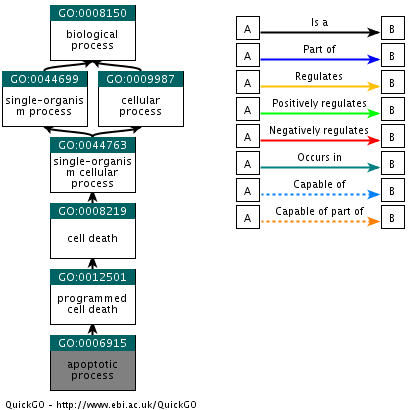
\includegraphics[width=\textwidth]{apoptotic.png}
        \caption{Relatively simplistic gene ontology (GO) term structure containing short and easily detected terminology.}
        \label{fig:simple}
    \end{subfigure}
    ~ 
    \begin{subfigure}[b]{0.45\textwidth}
        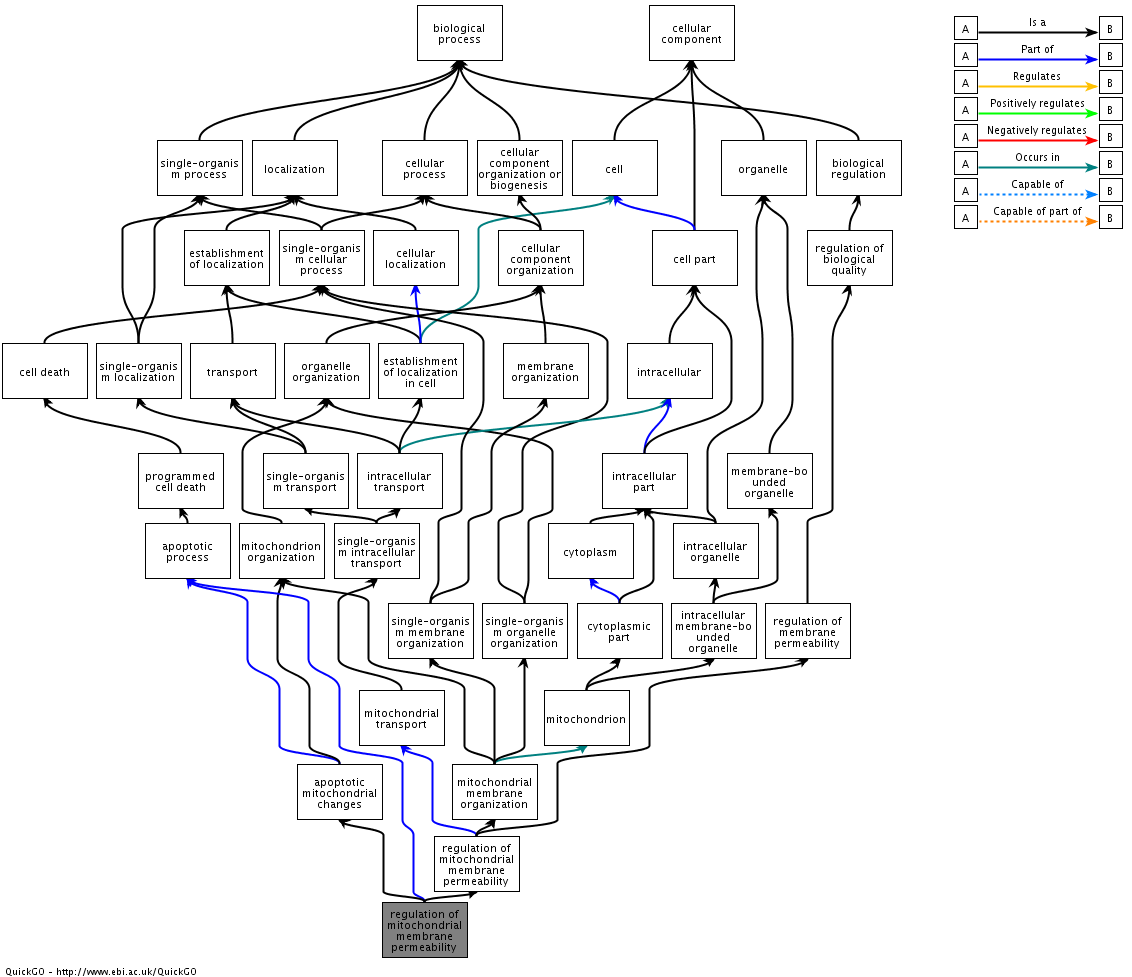
\includegraphics[width=\textwidth]{fig2.png}
        \caption{More complex gene ontology (GO) term structure containing highly specific and interrelated terminology.}
        \label{fig:complex}
    \end{subfigure}
    ~ 
    \caption{Examples of Gene Ontology Term Structures}\label{fig:animals}
\end{figure}

  
However, this structure quickly becomes unruly and complex once the specificity of a query increases. The corresponding strcture for the GO term ``regulation of mitochondrial membrane permeability involved in apoptotic process'' (GO:1902108) is displayed in \textbf{Figure 1b.}

A common application of this data is text mining. A researcher may wish to find common ``terms'' amongst a particular query on Pubmed. For example, a research group may want to identify common GO terms amonst a Pubmed Central (PMC) query for Alzheimers. PMC would return a list of publications which relate to Alzheimers, and the researcher aims to identify common or overrepresented GO terms in this corpus. The researcher would run into several problems.

\begin{enumerate}
\item Identifying a method to find co-occuring words which constitute a ``term'' and allowing the degree of confidence to vary by application.
\item Efficiently computing associations across hundreds or thousands of documents in a corpus.
\item Quantifying, summarizing, and reporting of associations in a meaninful way. 
\item Applying strict quality control and canonical natural language processing filters to improve true positive rate (TPR) and reduce false positive rate (FPR).
\end{enumerate}

In this article we present mineR as an R package capable of addressing these concerns and performing multi word term identification and quantification in natural langauge. We additionally develop methods for identifying and accounting for acronyms and synonyms by leveraging domain specific user knowledge.

\subsubsection{Design Philosophy}

In the framework proposed by Krauthammer \& Nenadić (\textbf{Figure 2.}), mineR lies firmly within the bounds of term recognition; other tools have been designed which excel at categorization and mapping, and as such the job of mineR ends after terms have been identified, summarized, and quantified. 

\begin{figure}[h]
\centering
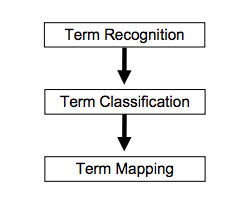
\includegraphics[width=0.5\textwidth]{fig3.png}
\caption{Term identification framework proposed by Krauthammer \& Nenadić (2004).}
\end{figure}

The failures of recent text mining approaches in the biomedical literature have largely revolved around a large disconnect between general methodologies such as those employed by TensorFlow and domain specific knowledge which is needed to accurately understand free language. Though this is a significant issue in all fields, it is especially apparent in biology and genetics where non-dictionary terms and acronyms are the majority rather than a small portion; computational algorithms struggle without a clear cut set of rules in these cases.

mineR attempts to address these concerns by requireing human knowledge and domain specific information to function. As an example, the strength and flexibility of mineR scales with the amount of time invested by the user constructing appropriate lists of synonyms, acronyms, and negations. Though this requires a larger time investment up front, the benefits are large. We hope that these lists of synonyms, acronyms, and negations will become public knowledge and posted on public databases such as our Github project site. 


\subsubsection{Typical Usage}

A typical analysis conducted with \mintinline{R}{mineR} is presented in supplemental methods 1: Basic Usage. However, here we present the rationale for any typical analysis. 

Firstly a user must identify and supply a list of terms which they are interested in analysing. For gene ontology based analyses, these may be found online. For others, users will have to defer to their specific area of expertise. Examples include mining publically available government documents for long program names, mining publically available literature for thematic expressions, and mining social media such as Twitter for ideas (``Rooney scored against Real Madrid''). 

Alongside this list of terms, the user must supply a single document or a corpus of documents to mine. These documents represent the sample space of the analysis.

From this, \mintinline{R}{mineR} will identify:

\begin{itemize}
\item Term's Frequency
\item Places within document where the term was identified
\item A term's relative importance

\end{itemize}

We note that \mintinline{R}{mineR} is usually, though not always, incompatible with latent semantic analysis because a large portion of its utility derives from breaking LSA's assumption that similar words appear in similar texts. For a large body of academic text this is not the case.

\subsubsection{Algorithm}

In general, the algorithm consists of the following steps.

\begin{enumerate}
\item Open connections to desired text, term list, and any other auxillary information like synonyms.
\item Split text into $n$ chunks to optimize processing.
\item (Optionally distribute $n$ chunks over $k$ computational cores).
\item Perform quality control (as detailed in iv.)
\item Construct term document matrix (TDM) of text, terms, and synonyms.
\item Account for synonyms and acronyms by adjusting TDM of terms.
\item Match counts from text TDM and term TDM.
\item Apply thresholding.
\item (Optionally summarize over multiple texts in a corpus).
\item Summarize, format, and return results of associations.
\end{enumerate}

To go into slightly more detail, connections to the text (or corpus) being mined are opened and converted from PDF or XML to a flat text document and stored within R as a vector, of which each element is a sentence delimited by a terminal punctuation mark (\mintinline{bash}{.!?}).  This vector has its whitespace cleared (a vestige from page breaks in the conversion process) and quality control measures are applied on the free text in order to reduce false positives and increase the discriminative power. Once the quality control measures (detailed in iv.) have been applied, a term document matrix (TDM) is constructed using the \mintinline{R}{tm} and \mintinline{R}{nlp} packages. Presently no transformations are applied to the TDM in order to alleviate any implicit assumptions on the goals of the term identification, though this will be the subject of future development and optional algorithms. An example of a TDM is displayed in \textbf{Figure 3.} This TDM is split into $n$ chunks to facilitate either parrelell (through \mintinline{R}{doParrelell} and \mintinline{R}{mcSnow}) or reduced serial computation time. 

\begin{figure}[h]
\centering
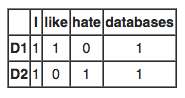
\includegraphics[width=0.25\textwidth]{fig4.png}
\caption{Example of a Term Document Matrix (TDM) for two sentences. ``D1'': I love databases, ``D2'': I hate databases.}
\end{figure}

After the term document transformation has been applied to the text, a similar transformation is applied to both the term list and the any synonyms which are presented to mineR. This is in order to standardize the quality control procedures to faciliate comparissons. 

We then merge the TDMs of the terms and the text to create a smaller TDM only looking at the specific words found in the term list. We augment this term list to indicate not only if a word in a term is present, but also if a synonym of that word is found. 

We then filter this matrix to include only the matches for one single term. We then take the row sums to be the number of words matched in a particular sentence from that specific term. We denote this as $s_i$.  From this, we must decide is $S_i$ is large enough to declare that a particular term $t_i$ is found in a particular sentence $s_i$.

This is accomplished through a user defined discontinuous step function which we call the acceptance function. By default we have defined the acceptence function $a$ as a function of $n$, the number of non-trivial words in a term such that 

$$  a(n) = \begin{cases} n, & 1 < n \leq 4 \\ n-1, & 5 < n < 8 \\ n-2, & 9 < n < 10 \\ 10, & n > 10 \end{cases} $$

If the number of words from the term present in a particular sentence exceeds $a(n)$, we call it a hit and say that the term was identified in that particular sentence. 

To summarize, we count up all sentences which have had a ``hit'' identified and diaplay this information collapsed over terms. This information may be meta analyzed over a corpus or between corpi for comparitive analyses. 

\subsubsection{Quality Control}

\texttt{mineR} incorporates many standard quality control procedures common to many NLP analysis pipelines. These include:

\begin{itemize}
  \item Case standardization
  \item Punctuation elimination (with exception cases)
  \item Numerical elimination (with exception cases)
  \item Removing of Stop Words (for a given language, or standard english by default)
  \item Consistent word stemming
  \item Whitespace elimination and consideration
  \item Term Document Matrix (TDM) creation and reporting and frequency reporting
\end{itemize}

Given an input document or corpus of documents in PDF form and a text encoding format, \texttt{mineR} will convert documents in PDF form to plain text.  If the user is unsure of formatting, \texttt{mineR} will by default guess at the formatting. Preliminary QC is performed on the documents through case standardization, punctuation elimination, numerical elimination, and the removal of stop words.  The document is then stemmed, and white space is eliminated.

A similar process is conducted on the input list of terms, given one per line with unix return characters in a specified plain text document. The terms are then standardized to match the format of text in the document by the above mentioned steps.

\subsubsection{Computational Considerations}

As the number of terms increases, the computational time that the algorithm wil require increases expodentially (\textbf{Figure 4.}).

\begin{figure}[h]
\centering
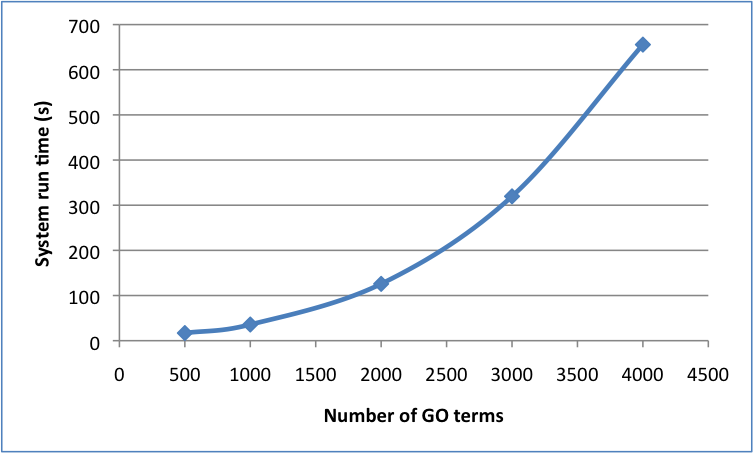
\includegraphics[width=0.6\textwidth]{GO_np.png}
\caption{\mintinline{R}{mineR} run time to completion in seconds performed on a MacBook Pro OSX v10.9.5 with a 2.66 GHz Intel Core 2 Duo processor and 4 GB 1067 MHz DDR3 RAM.}
\end{figure}

Users are encouraged to take advantage of this behaviour and chunk terms into batches of 100-500 terms to make computational time reasonable. \mintinline{R}{mineR} includes an option to guide the user through this process, see \mintinline{R}{?mineR::term_chunk()} for details.

\subsection{Implimentation and Architechture}

\mintinline{R}{mineR} is written in native R scripts with no compilation of other languages. It heavily uses the following packages:

 \begin{enumerate}
\item \mintinline{R}{tm}
\item \mintinline{R}{Rcpp}
\item \mintinline{R}{dplyr}
\item \mintinline{R}{SnowballC}
\item \mintinline{R}{foreach}

\end{enumerate}

Known functional versions of these libraries have been included in a \mintinline{R}{packrat} personalized CRAN instanced bundled along with \mintinline{R}{mineR}.

\mintinline{R}{mineR} contains one overarching function \mintinline{R}{mineR::mineR()} which takes two mandatory arguements, \mintinline{R}{doc} and \mintinline{R}{terms}, containing a .pdf or .txt file and a \mintinline{bash}{\n} delimited list of terms to be identified. A brief example is given below in Usage Instructions and a more complete runthrough with examples and explaination is given in the ``Basic Usage'' vignette, also supplemental methods 1. 

\mintinline{R}{mineR} only uses one core by default, but may be multi corred by setting \mintinline{R}{mc.cores = n} where $n$ is the number of cores you want to use. This will additionally import \mintinline{R}{doMC} and register the local parrellel backend. Keep in mind that your milage may vary with parrellel computing depending on the size of your data set; for small sets of terms and/or small files, parrellizing may actually slow down computational speeds due to the relatively quick iterations performed and the increased load of distributing and balancing jobs over the backbone. 

\mintinline{R}{mineR} is designed to be used in batch operations, however for smaller scale or pilot testing, an interaction version may be used, in which the program guides the user through the logic and process of designing their terms and synonyms. This may be performed by giving \mintinline{R}{``interactive''} to any of \mintinline{R}{lims}, \mintinline{R}{syn} or \mintinline{R}{acro}, which will call \mintinline{R}{mineR::make.lims}, \mintinline{R}{mineR::make.syn}, and \mintinline{R}{mineR::make.acro} respectively. 

Optionally, a log file may be written to the path specified to the log \mintinline{R}{log = ``path''}, or if \mintinline{R}{log = TRUE} then \mintinline{R}{mineR} will write to \mintinline{sh}{mineR.txt} in the current working directory. 

A full descriptions of arguements for the \mintinline{R}{mineR} is given in \textbf{Table 1}.

\subsection{Quality Control}

\mintinline{R}{mineR} impliments several layers of quality control. Firstly, we bundle with \mintinline{R}{mineR} a \mintinline{R}{packrat} personalized CRAN instance to control package dependencies and ensure that functions will work as expected. Unit testing is conducted on essential functions through the \mintinline{R}{testthat} package, with code coverage estimated at 57\% by \mintinline{R}{covr} at time of writing. 

Additionally, continuous integration is tested for each new release by Travis CI on OSX and linux, and through Appveyor for windows. 

Additionally, users may run 

\begin{minted}{R}
mineR::mineR(test = TRUE)
\end{minted}

with no additionally arguements to verify the complete function of the package. The function will return \mintinline{R}{TRUE} if all is working correctly, and \mintinline{R}{FALSE} if there are any errors. An attempt will be made to show at which portion the test failed.

\section{Availability}

\section{Reuse Potential}

Typical and expected use of \mintinline{R}{mineR} is in the mining of biomedical literature, specifically through Gene Ontology terms. However, we see potential for this software outside of biology in fields such as the humanities and social media text mining. We believe that the identification of key terms is a fairly general process which may be applied in many areas, many of which we are unaware. Additionally, the code contained in this package may be included in different applications and software to incorporate the method into new areas. 

\section{References}

\todo[inline]{Add in references}


\newpage
\listoftodos[Notes]

\end{document}
